\documentclass[../SWD_disp.tex]{subfiles}

\begin{document}
\section{Factory Patterns}
\begin{enumerate}
    \item Factory - Wholesale creation
    \item Abstract Factory - Objects in hierarchies
\end{enumerate}

Redegøre for opbygningen af GoF Fatory og Abstract Factory Pattern.
\\

De to patterns hører til Creational Patterns kategorien, hvor deres generelle ide er faktorisering ved at sepererer oprettelse af objektet fra dens anvendelse. De bruges til at kontrollerer klasse initialisering.

\subsection*{Factory Pattern}
Dette pattern definerer et interface for oprettelse af objektet, man lader klassen der implementerer interfacet bestemmet, hvilket objekt der skal oprettes. Dvs. at den i princippet er en udskifter for en klasse constructor.

\begin{figure}[H]
    \centering
    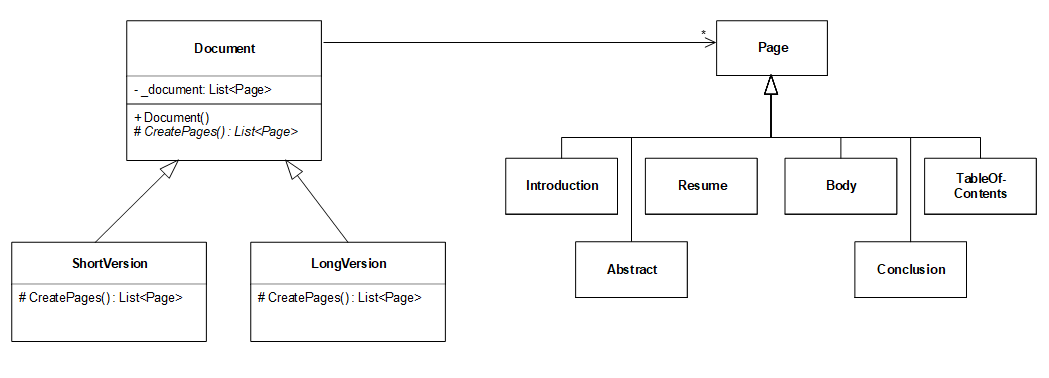
\includegraphics[width = \textwidth]{factory_pattern.PNG}
\end{figure}

Definerer et interface ud fra \textbf{CreatePage()}, men lader klasserne der implementerer interfacet bestemme hvilket objekt der skal oprettes. Den abstrakte klasse vil blive anvendt således, at andre funktioner kan modtages ved arv af subklasserne.

\subsection*{Abstract Factory Pattern}
I modsætning til det almene factory vist tidligere, så understøtter et abstract factory et pattern som kan retunere et nyt factory. Dette betyder altså at du kan retunere et factory fra et factory. 

antag vi har en abstract klasse HotDrink. Dette er en form for varm drikkelse. Vi vil have mulighed for at lave både Kaffer og Te af vores hotdrinks, men kun en ting af gangen. 

Forestil dig er der er 15 forskellige typer af både kaffe og te. Interfaces HotDrinkFactory er det abstracte factory. Dette er altså bare en måde at sige, lige meget hvilket factory som arver fra mig, så kan du få det. 

Lad os så antage at jeg ville have en kop dejlig Espresso, så skal jeg altså lave et nyt 
\mint{typescript}|coffeeFac: HotDrinkFactory = new CoffeeFactory()|
Her antages det at der hvor vores factory skal bruges, at der findes en parameter HotDrinkFactory. 

Alternativt kan der laves en ny klasse til at encapsulere både vores te og kaffe factories kaldet DrinkFactory. Så kan der kaldes direkte på dem: 
Nu kan vi enten ved at kalde make med den kaffe eller te vi vil have, også få det rette object tilbage.

\begin{minted}{typescript}
export class DrinkFactory {

    public coffee: CoffeeFactory;
    public tea: TeaFactory;

    constructor() {
        this.coffee = new CoffeeFactory();
        this.tea = new TeaFactory();
    }
}
\end{minted}

Dette kan yderligere afkobles ved at bruge dependency inversion, og dependency inject de factories man skal bruge. På den måde kan drink factory understykke enhver 2 typer varme drinks. 

\begin{figure}[H]
    \centering
    \includegraphics[width = 0.5\textwidth]{abstract_factory.PNG}
\end{figure}

\end{document}
